\begin{question}
Using the Euler scheme, write a program to simulate:
\begin{itemize}
\tightlist
\item a Wiener process;
\item a Brownian motion with $S_0 = 100$, $\mu=0.05$ and $\sigma=0.17$;
\item the stock price following a Geometric Brownian motion with $S_0 = 100$, $\mu=0.05$ and $\sigma=0.17$.
\end{itemize}
\end{question}

\cprotEnv\begin{solution}
\begin{ipython}
from numpy.random import normal, seed
import numpy as np

S = 100
mu = 0.05
sigma = 0.17
T = 1
steps = 360

seed(1)
wiener = [S]
abm = [S]
gbm = [S]

for i in range(steps):
    wiener.append(wiener[-1] + normal()*np.sqrt(T/steps))
    abm.append(abm[-1] + mu * T/steps + sigma * np.sqrt(T/steps) * normal())
    S = S * np.exp((mu - 0.5 * sigma * sigma) * T/steps + sigma * \
                    np.sqrt(T/steps) * normal())
    gbm.append(S)
\end{ipython}

\begin{figure}[htbp]
\centering
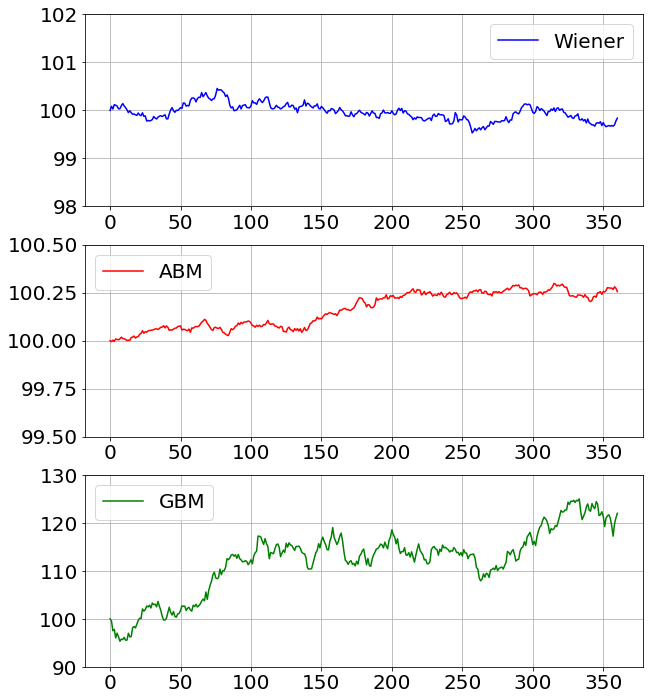
\includegraphics[width=0.5\linewidth]{figures/ex_stochastic}
\caption{Realizations of different kind of stochastic processes.}
\end{figure}
\end{solution}

\cprotEnv\begin{question}
Using the Euler scheme and a Monte Carlo simulation price an European vanilla call option

\begin{ipython}
S0 = 110
r = 0.05
sigma = 0.17
ttm = 1
K = 105
\end{ipython}

Plot the relative pricing difference (simulated price minus Black-Scholes price) versus the number of simulated scenarios (e.g. 10000 simulations).
Also measure the timing for the entire simulation and try to improve it.
\end{question}

\cprotEnv\begin{solution}
The reference price is the one computed using the Black-Scholes formula
\begin{ipython}
from finmarkets import call

S0 = 110
r = 0.05
sigma = 0.17
T = "1y"
K = 105

C0 = call(S0, K, r, sigma, T)

print ("BS call price: {:.2f}".format(C0))
\end{ipython}
\begin{ioutput}
BS call price: 13.28
\end{ioutput}

The first Monte Carlo implementation uses standard lists and for-loops
\begin{ipython}
import time
from math import exp, sqrt
from numpy.random import normal, seed

t1 = time.time()
S0 = 110
r = 0.05
sigma = 0.17
T = 1
K = 105

values = []
for sim in range(1, 10000):
  seed(sim)
  payoff = []
  for i in range(sim):
    St = S0 * exp((r - 0.5 * sigma * sigma) * T + sigma * sqrt(T) * normal())
    payoff.append(exp(-r*T)*max(0, St-K))
  values.append(sum(payoff)/sim)

Cs = []
for i in range(1, len(values)):
  Cs.append((sum(values[:i])/i - C0)/C0)

print ("Elapsed time: ", time.time() - t1)
\end{ipython}
\begin{ioutput}
Elapsed time:  296.0764889717102
\end{ioutput}

Plotting the relative difference between the MC and BS price it is apparent how the agreement improves as the number of simulations increases.

\begin{figure}[htbp]
\centering
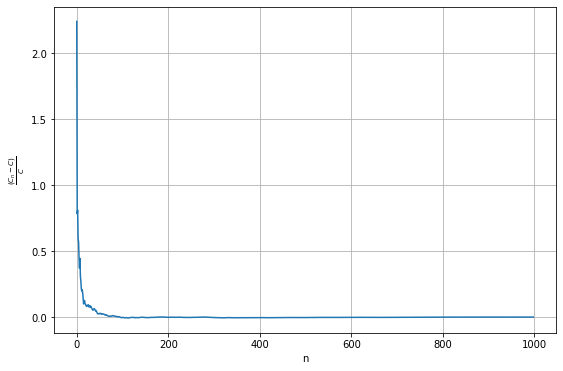
\includegraphics[width=0.7\linewidth]{figures/ex_call_pricing_error}
\caption{Call pricing difference as a function of the number of simulated scenarios.}
\end{figure}

The very same algorithm implemented using \texttt{numpy.array} is more concise, and more importantly, much faster since it runs in one hundredth of the time. Note that this is kind of cheating since we are relying on the \texttt{C} implementation underlying \texttt{numpy}.

\begin{ipython}
import numpy as np
import time
from scipy.stats import norm

t1 = time.time()
S0 = 110
r = 0.05
sigma = 0.17
T = 1
K = 105

Cs = []
for i in range(1, 10000):
  np.random.seed(i)
  Z = norm.rvs(size=i)
  St = S0 * np.exp((r - 0.5 * sigma ** 2) * T + sigma * np.sqrt(Tt) * Z)
  Cs.append(np.mean(np.exp(-r * T) * np.maximum(St - K, 0)))

n = 1/np.arange(1, 10000)
c = np.cumsum(Cs)*n

print ("Elapsed time: ", time.time() - t1)
\end{ipython}
\begin{ioutput}
Elapsed time:  4.282579183578491
\end{ioutput}
\end{solution}

\begin{question}
Assume that a man’s profession can be classified as professional, skilled labourer, or unskilled labourer. Assume that, of the sons of professional men, 80 percent are professional, 10 percent are skilled labourers, and 10 percent are unskilled labourers.

In the case of sons of skilled labourers, 60 percent are skilled labourers, 20 percent are professional, and 20 percent are unskilled. Finally, in the case of unskilled labourers, 50 percent of the sons are unskilled labourers, and 25 percent each are in the other two categories. Assume that every man has at least one son, and form a Markov chain by following the profession of a randomly chosen son of a given family through several generations. Set up the matrix of transition probabilities. Find the probability that a randomly chosen grandson of an unskilled labourer is a professional man.
\end{question}

\cprotEnv\begin{solution}
The Markov chain in this exercise has the following set states
\begin{equation*}
S = \{\textrm{Professional, Skilled, Unskilled}\}
\end{equation*}
with the following transition probabilities:

\begin{table}[htbp]
\centering
\begin{tabular}{l c c c}
&Professional& Skilled &Unskilled \\
Professional & .8 & .1 & .1 \\
Skilled & .2 & .6 & .2 \\
Unskilled & .25 & .25 & .5 \\
\end{tabular}
\end{table}
\noindent
so that the transition matrix for this chain is

\begin{equation*}
\Pi =
\begin{bmatrix}
.8 &.1 &.1\\
.2 &.6 &.2\\
.25 &.25 &.5
\end{bmatrix}
\end{equation*}

Since we are interested to find the probability that a grandson of an unskilled labourer is a professional we need to apply twice the transition matrix to the initial state $C=(0, 0, 1)$.
\begin{ipython}
import numpy as np

C = np.array([0,0,1])
P = np.array([[.8, .1,.1],[.2,.6,.2],[.25,.25,.5]])

C_grandson = C.dot(P).dot(P)
print (C_grandson[0])
\end{ipython}
\begin{ioutput}
0.375
\end{ioutput}
\end{solution}

\begin{question}
Consider an experiment of mating rabbits. We watch the evolution of a particular gene that appears in two types, $G$ or $g$. A rabbit has a pair of genes, either $GG$ (dominant), $Gg$ (hybrid, the order is irrelevant, so $gG$ is the same as $Gg$) or gg (recessive).

In mating two rabbits, the offspring inherits a gene from each of its parents with equal probability. Thus, if we mate a dominant ($GG$) with a hybrid ($Gg$), the offspring is dominant with probability 1/2 or hybrid with probability 1/2.
Start with a rabbit of given character ($GG$, $Gg$, or $gg$) and mate it with a hybrid. The offspring produced is again mated with a hybrid, and the process is repeated through a number of generations, always mating with a hybrid.
\begin{tasks}
\task Write down the transition probabilities of the Markov chain thus defined;
\task assume that we start with a hybrid rabbit. Let $\mu_n$ be the probability distribution of the character of the rabbit of the n$^{th}$ generation. In other words, $\mu_n(GG)$, $\mu_n(Gg)$, $\mu_n(gg)$ are the probabilities that the n$^{th}$ generation rabbit is $GG$, $Gg$, or $gg$, respectively. Compute $\mu_1$, $\mu_2$, $\mu_3$.
\end{tasks}
\end{question}

\cprotEnv\begin{solution}
The set of states is 
\begin{equation*}
S = \{\textrm{GG, Gg, gg}\}
\end{equation*}
with the following transition probabilities:

\begin{table}[htbp]
\centering
\begin{tabular}{l c c c}
&GG& Gg & gg \\
GG & .5 & .5 & 0 \\
Gg & .25 & .5 & .25 \\
gg & 0 & .5 & .5 \\
\end{tabular}
\end{table}
\noindent
We can rewrite the transition matrix in the following form:

\begin{equation*}
\Pi =
\begin{bmatrix}
.5 &.5 &0\\
.25 &.5 &.25\\
0 &.5 &.5
\end{bmatrix}
\end{equation*}

The elements from the second row of the matrix $\Pi^n$ will give us the probabilities for a hybrid to give dominant, hybrid or recessive species in $(n − 1)^{th}$ generation in this experiment, respectively (reading this row from left to right).
\begin{ipython}
import numpy as np

P = np.array([[.5,.5,0],[.25,.5,.25],[0,.5,.5]])

mu1 = P[1, :]
mu2 = P.dot(P)[1, :]
mu3 = P.dot(P).dot(P)[1, :]

print (mu1)
print (mu2)
print (mu3)
\end{ipython}
\begin{ioutput}
[0.25 0.5  0.25]
[0.25 0.5  0.25]
[0.25 0.5  0.25]
\end{ioutput}
so that $\mu_i(GG) = .25, \mu_i(Gg) = .5, \mu_i(gg) = .25$, $i = 1, 2, 3$.
Actually the probabilities are the same for any $i \in \mathbb{N}$. 

\begin{curiosity}
If you obtained this result before 1858 when Gregor Mendel started to breed garden peas in his monastery garden and analysed the offspring of these matings, you would probably be very famous because it definitely looks like a law! This is what Mendel found when he crossed mono-hybrids.
\end{curiosity}
\end{solution}
